% !TeX program = xelatex
\documentclass[a4paper,10pt]{article}

% ============================================================================
% សន្លឹកកិច្ចការសិស្សបំពេញចន្លោះ ស-ខ្មៅ និងប្លង់ក្ដារខៀន/ចម្លើយគ្រូ (គ្មាន LCD / គ្មានកន្ត្រៃ)
% មេរៀនទី១ (៥.)៖ លក្ខណៈនៃប្រមាណវិធីបូកនិងគុណ — ត្រូវគ្នា ១០០% នឹង LS_Plan_WN14.tex
% ============================================================================
\usepackage[a4paper, left=1.0cm, right=1.0cm, top=0.75cm, bottom=1.00cm, footskip=0.52cm]{geometry}
\usepackage{amsmath}
\usepackage{unicode-math}
\usepackage{fontspec}
\usepackage{array, colortbl}
\usepackage[table]{xcolor}
\usepackage{enumitem}
\usepackage{pifont}
\usepackage{fancyhdr}
\usepackage{lastpage}
\usepackage{tikz}
\usepackage[most]{tcolorbox}
\usetikzlibrary{calc, arrows.meta, decorations.pathreplacing, positioning, babel}

\makeatletter
\let\@expl@@@mark@update@singlecol@structures@@\relax
\makeatother

\providecommand{\NGSFindFonts}{%
  \IfFileExists{C:/Windows/Fonts/cambria.ttc}{%
    \def\NGSSysPath{C:/Windows/Fonts/}%
    \def\NGSUserPath{C:/Users/KIT/AppData/Local/Microsoft/Windows/Fonts/}%
  }{%
    \IfFileExists{./fonts/KhmerOSsiemreap.ttf}{\def\NGSSysPath{./fonts/}\def\NGSUserPath{./fonts/}}{%
    \IfFileExists{../fonts/KhmerOSsiemreap.ttf}{\def\NGSSysPath{../fonts/}\def\NGSUserPath{../fonts/}}{%
    \IfFileExists{../../fonts/KhmerOSsiemreap.ttf}{\def\NGSSysPath{../../fonts/}\def\NGSUserPath{../../fonts/}}{%
    \IfFileExists{../../../fonts/KhmerOSsiemreap.ttf}{\def\NGSSysPath{../../../fonts/}\def\NGSUserPath{../../../fonts/}}{%
    \IfFileExists{../../../../fonts/KhmerOSsiemreap.ttf}{\def\NGSSysPath{../../../../fonts/}\def\NGSUserPath{../../../../fonts/}}{%
    \IfFileExists{../../../../../fonts/KhmerOSsiemreap.ttf}{\def\NGSSysPath{../../../../../fonts/}\def\NGSUserPath{../../../../../fonts/}}{%
    \IfFileExists{../../../../../../fonts/KhmerOSsiemreap.ttf}{\def\NGSSysPath{../../../../../../fonts/}\def\NGSUserPath{../../../../../../fonts/}}{%
      \def\NGSSysPath{../../../../../../../fonts/}\def\NGSUserPath{../../../../../../../fonts/}%
    }}}}}}}%
  }%
}
\NGSFindFonts

\setmathfont[Path={\NGSSysPath}, FontIndex=1, Scale=1.02]{cambria.ttc}
\defaultfontfeatures{Ligatures=TeX}

\setmainfont[
  Path={\NGSUserPath}, Extension=.ttf, Script=Khmer,
  BoldFont={KhmerOSsiemreap}, BoldFeatures={FakeBold=1.8},
  ItalicFont={KhmerOSsiemreap}, ItalicFeatures={FakeSlant=0.25},
  BoldItalicFont={KhmerOSsiemreap}, BoldItalicFeatures={FakeBold=1.8, FakeSlant=0.25}
]{KhmerOSsiemreap}

\newfontfamily\muol[Path={\NGSUserPath}, Extension=.ttf, Script=Khmer]{KhmerOSmuollight}
\newfontfamily\TimesEn[Path={\NGSSysPath}, Extension=.ttf, BoldFont={timesbd}, ItalicFont={timesi}, BoldItalicFont={timesbi}]{times}
\newfontfamily\CalibriFont[Path={\NGSSysPath}, Extension=.ttf]{calibri}

\XeTeXlinebreaklocale "km"
\XeTeXlinebreakskip = 0pt plus 1pt minus 0.1pt

\definecolor{panelgray}{gray}{0.94}
\definecolor{headgray}{gray}{0.85}

\pagestyle{fancy}
\fancyhf{}
\renewcommand{\headrulewidth}{0pt}
\fancyfoot[L]{\fontsize{7.4pt}{9.5pt}\selectfont អនុវិទ្យាល័យព្រះក្រសាំង \en{|} គ្រូ៖ ហុក ប៊ុនថែន \en{|} មេរៀនទី១ (៥.) លក្ខណៈនៃប្រមាណវិធី \en{|} ថ្ងៃសុក្រ ទី៦ ខែវិច្ឆិកា ឆ្នាំ២០២៦}
\fancyfoot[R]{\fontsize{7.8pt}{10pt}\selectfont ទំព័រ \en{\thepage\ / \pageref{LastPage}}}

\setlength{\parindent}{0pt}
\setlength{\parskip}{0pt}
\setlength{\tabcolsep}{4pt}
\newcolumntype{L}[1]{>{\raggedright\arraybackslash}p{#1}}
\newcolumntype{C}[1]{>{\centering\arraybackslash}p{#1}}

\newcommand{\en}[1]{{\TimesEn #1}}
\newcommand{\enbf}[1]{{\TimesEn\bfseries #1}}
\newcommand{\unit}[1]{\,\text{\en{#1}}}
\newcommand{\cnum}[1]{\mbox{\fontsize{10pt}{12pt}\selectfont\ding{\numexpr181+#1\relax}}}
\newcommand{\chkbox}{\tikz[baseline=-0.15ex]\draw[black, line width=0.85pt, fill=white] (0,0) rectangle (0.24cm,0.24cm);}
\newcommand{\ansbox}[1][1.75cm]{\,\tikz[baseline=-0.65ex]\draw[black, line width=0.65pt, fill=white] (0,0) rectangle (#1, 0.42cm);\,}
\newcommand{\dotline}[1][2.2cm]{\makebox[#1]{\dotfill}}

\newcommand{\pagebanner}[2]{%
  \begin{tcolorbox}[
    enhanced, sharp corners, colback=headgray, colframe=black,
    boxrule=1.05pt, boxsep=1pt, top=2.5pt, bottom=2.5pt, left=6pt, right=6pt,
    after skip=3.5pt
  ]
    {\muol\fontsize{9.0pt}{13.2pt}\selectfont #1}\hfill{\fontsize{8.0pt}{11.2pt}\selectfont\textbf{#2}}
  \end{tcolorbox}%
}

\newcommand{\secstrip}[2]{%
  \vspace{3pt}%
  \begin{tcolorbox}[
    enhanced, sharp corners, colback=panelgray, colframe=black,
    boxrule=0.8pt, boxsep=0.8pt, top=2pt, bottom=2pt, left=5pt, right=5pt,
    after skip=3pt
  ]
    {\muol\fontsize{8.5pt}{12.2pt}\selectfont #1}\hfill{\fontsize{7.8pt}{10.8pt}\selectfont\textit{#2}}
  \end{tcolorbox}%
}

\begin{document}
\fontsize{9.5pt}{14.5pt}\selectfont

% ============================================================================
% ទំព័រទី ១៖ សន្លឹកកិច្ចការសិស្ស (ផ្នែកមុខ៖ E1 -> E2 -> E3)
% ============================================================================
\pagebanner{សន្លឹកកិច្ចការសិស្ស \enbf{(}៥\enbf{.} លក្ខណៈនៃប្រមាណវិធីបូកនិងគុណ\enbf{)} \enbf{--} ផ្នែកមុខ}{ថ្នាក់ទី៧ \en{|} សៀវភៅគោល ទំ.៦--៨}

\begin{tcolorbox}[
  enhanced, sharp corners, colback=white, colframe=black,
  boxrule=0.8pt, boxsep=1.5pt, top=3.5pt, bottom=3.5pt, left=5pt, right=5pt,
  after skip=4pt
]
  \fontsize{9.0pt}{13.0pt}\selectfont
  \textbf{ឈ្មោះសិស្ស៖} \dotline[4.3cm] \quad
  \textbf{សមាជិកក្រុម៖} \dotline[4.3cm] \quad
  \textbf{ថ្នាក់ទី៖} ៧\dotline[0.9cm] \quad
  \textbf{ក្រុមទី៖} \dotline[1.0cm]
\end{tcolorbox}

% --- E1 Engage ---
\secstrip{ផ្នែកទី ១ \enbf{(E1 - Engage)} ៖ បេសកកម្មអន្ទាក់ការបំបែក $6 \times (3 + 4)$}{រយៈពេល ៣ នាទី (គូស \ding{51} ក្នុង \chkbox)}

\begin{tcolorbox}[
  enhanced, sharp corners, colback=white, colframe=black,
  boxrule=0.8pt, boxsep=2pt, top=4pt, bottom=4pt, left=6pt, right=6pt
]
  គេរៀបការ៉ូជា $6$ ជួរដេក ដែលក្នុង ១ ជួរដេកមានការ៉ូស $3$ និងការ៉ូប្រផេះ $4$ ពោលគឺ $6 \times (3 + 4)$ (ឧទាហរណ៍ ៣ ទំ.៨)៖\\[3pt]
  $\bullet$ \textbf{តើសិស្សរូបណាបំបែកផលគុណបានត្រឹមត្រូវ?} \quad
  \chkbox\ \textbf{សិស្ស ក៖} $6 \times 3 + 4 = 22$ \quad
  \chkbox\ \textbf{សិស្ស ខ៖} $(6 \times 3) + (6 \times 4) = 42$\\[3pt]
  $\bullet$ \textbf{ហេតុផល៖} កត្តា $6$ ត្រូវគុណនឹងតួក្នុងវង់ក្រចកចំនួន \dotline[1.2cm] តួ ស្មើនឹង $6 \times 7 =$ \dotline[1.4cm] ការ៉ូ ។
\end{tcolorbox}

\vfill

% --- E2 Explore ---
\secstrip{ផ្នែកទី ២ \enbf{(E2 - Explore)} ៖ លក្ខណៈវិធីបូក និងរូបក្រឡាការ៉ូលក្ខណៈវិធីគុណ (ទំ.៦--៨)}{រយៈពេល ១១ នាទី}

\textbf{សកម្មភាព ១ (\en{E2-A} — ៥ នាទី)៖ លក្ខណៈនៃវិធីបូក និងវិធីគុណ — ត្រឡប់ ផ្ដុំ និងធាតុណឺត (ទំ.៦--៨)}

\begin{tcolorbox}[
  enhanced, sharp corners, colback=white, colframe=black,
  boxrule=0.8pt, boxsep=2.5pt, top=4.5pt, bottom=4.5pt, left=6pt, right=6pt
]
  $\bullet$ \textbf{៥.១ វិធីបូក (ទំ.៦--៧)៖} ១) $4+5 = 5+4 =$ \dotline[0.9cm] (ត្រឡប់) $\mid$ ២) $(2+3)+5 = 2+(3+5) =$ \dotline[1.0cm] (ផ្ដុំ) $\mid$ ៣) $1+0 = 0+1 =$ \dotline[0.9cm]\\[3.5pt]
  $\bullet$ \textbf{៥.២ វិធីគុណ (ទំ.៧--៨)៖} ១) $7\times 5 = 5\times 7 =$ \dotline[1.0cm] $\mid$ ២) $5\times(3\times 4) = 4\times(3\times 5) =$ \dotline[1.0cm] $\mid$ ៣) $1\times 14 = 14\times 1 =$ \ansbox[1.3cm]
\end{tcolorbox}

\vspace{4pt}
\textbf{សកម្មភាព ២ (\en{E2-B} — ៦ នាទី)៖ រូបក្រឡាការ៉ូបំបែកនៃវិធីគុណចំពោះវិធីបូក (ឧទាហរណ៍ ៣ ទំ.៨)}

\begin{tcolorbox}[
  enhanced, sharp corners, colback=white, colframe=black,
  boxrule=0.8pt, boxsep=2.5pt, top=4.5pt, bottom=4.5pt, left=6pt, right=6pt
]
  \begin{minipage}{5.6cm}
    \centering
    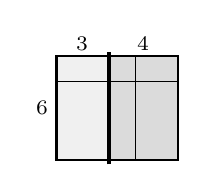
\begin{tikzpicture}[x=0.22cm, y=0.22cm, every node/.style={font=\fontsize{7.5pt}{9.5pt}\selectfont, text=black}]
      \fill[gray!12] (0,0) rectangle (3,6);
      \fill[gray!28] (3,0) rectangle (7,6);
      \draw[black, line width=0.35pt] (0,0) grid (7,6);
      \draw[black, line width=0.9pt] (0,0) rectangle (7,6);
      \draw[black, line width=1.4pt] (3,-0.25) -- (3,6.25);
      \node at (-0.8,3) {$6$};
      \node at (1.5,6.7) {$3$};
      \node at (5.0,6.7) {$4$};
    \end{tikzpicture}
  \end{minipage}\hfill
  \begin{minipage}{12.5cm}
    $\bullet$ គណនាតាមចំនួនជួរឈរសរុប៖ $6 \times (3 + 4) = 6 \times$ \dotline[1.0cm] $=$ \ansbox[1.5cm] ការ៉ូ\\[3.5pt]
    $\bullet$ គណនាតាមផ្នែកទាំងពីរ៖ $(6 \times 3) + (6 \times 4) =$ \dotline[1.1cm] $+$ \dotline[1.1cm] $=$ \ansbox[1.5cm] ការ៉ូ\\[3.5pt]
    $\bullet$ សន្និដ្ឋាន៖ $6 \times (3 + 4) = (6 \times$ \dotline[0.9cm] $) + (6 \times$ \dotline[0.9cm] $)$ ។
  \end{minipage}
\end{tcolorbox}

\vfill

% --- E3 Explain ---
\secstrip{ផ្នែកទី ៣ \enbf{(E3 - Explain)} ៖ រូបមន្តជាទូទៅ និងធនាគារហេតុផល \enbf{B\&W}}{រយៈពេល ៦ នាទី}

\begin{tcolorbox}[
  enhanced, sharp corners, colback=white, colframe=black,
  boxrule=0.85pt, boxsep=2.5pt, top=4pt, bottom=4pt, left=6pt, right=6pt
]
  ចំពោះគ្រប់ចំនួនគត់ $a, b, c$៖ \quad
  ១) ធាតុណឺតវិធីបូកគឺ \dotline[0.8cm] ($a+0=a$) \quad
  ២) ធាតុណឺតវិធីគុណគឺ \dotline[0.8cm] ($a\times 1=a$)\\[3pt]
  ៣) លក្ខណៈបំបែកនៃវិធីគុណចំពោះវិធីបូក៖ $a(b + c) = (a \times$ \dotline[0.8cm] $) + (a \times$ \dotline[0.8cm] $)$ \quad (ចំពោះវិធីដក៖ $a(b-c)=ab-ac$)\\[4pt]
  \tikz\draw[black, dashed, line width=0.5pt] (0,0) -- (18.4cm,0);\\[3.5pt]
  \fontsize{8.8pt}{13.0pt}\selectfont
  \textbf{ធនាគារហេតុផល (\en{Warrant Bank})៖} \quad
  \cnum{1} \textbf{លក្ខណៈត្រឡប់៖} $a+b=b+a, \ ab=ba$ \quad
  \cnum{2} \textbf{លក្ខណៈផ្ដុំ៖} $(a+b)+c=a+(b+c), \ (ab)c=a(bc)$\\
  \cnum{3} \textbf{លក្ខណៈបំបែក៖} $a(b\pm c) = ab \pm ac$ (គុណគ្រប់តួក្នុងវង់ក្រចក) \quad
  \cnum{4} \textbf{ធាតុណឺត៖} $0$ ចំពោះវិធីបូក; $1$ ចំពោះវិធីគុណ (ឯ $a\times 0 = 0$)
\end{tcolorbox}

% ============================================================================
% ទំព័រទី ២៖ សន្លឹកកិច្ចការសិស្ស (ផ្នែកខាងខ្នង៖ E4 -> E5 -> កិច្ចការផ្ទះ)
% ============================================================================
\clearpage
\pagebanner{សន្លឹកកិច្ចការសិស្ស \enbf{(}៥\enbf{.} លក្ខណៈនៃប្រមាណវិធីបូកនិងគុណ\enbf{)} \enbf{--} ផ្នែកខាងខ្នង}{ថ្នាក់ទី៧ \en{|} សៀវភៅគោល ទំ.៨--៩ និង ទំ.១៤}

% --- E4 Elaborate ---
\secstrip{ផ្នែកទី ៤ \enbf{(E4 - Elaborate)} ៖ លំហាត់គំរូ — ចំណោទចានកូនឃ្លី (សៀវភៅគោល ទំ.៨)}{រយៈពេល ១០ នាទី}

\begin{tcolorbox}[
  enhanced, sharp corners, colback=white, colframe=black,
  boxrule=0.8pt, boxsep=2.5pt, top=4.5pt, bottom=4.5pt, left=6pt, right=6pt
]
  \textbf{លំហាត់គំរូ (ទំ.៨)៖} ចានមួយមានកូនឃ្លីច្រើនជាង $80$ គ្រាប់ ប៉ុន្តែតិចជាង $90$ គ្រាប់ ហើយវាស្មើនឹង $7$ ដងនៃផលបូកតួលេខនៃចំនួនឃ្លីទាំងអស់ ។ តើកូនឃ្លីសរុបដែលនៅក្នុងចានមានចំនួនប៉ុន្មានគ្រាប់?\\[3.5pt]
  $\bullet$ \textbf{ជំហានទី១ (កំណត់លក្ខខណ្ឌ)៖} តាង $n$ ជាចំនួនគ្រាប់ឃ្លីទាំងអស់ ដែល $80 < n < 90$ ហើយ $n$ ត្រូវជាពហុគុណនៃ $7$ ។\\[3pt]
  $\bullet$ \textbf{ជំហានទី២ (ផ្ទៀងផ្ទាត់តម្លៃ)៖} បើ $n = 81 \implies (8+1)\times 7 =$ \dotline[1.1cm] $\ne 81$; \quad បើ $n = 84 \implies (8+4)\times 7 =$ \dotline[1.1cm] $\times 7 =$ \ansbox[1.5cm]\\[3pt]
  $\bullet$ \textbf{សន្និដ្ឋាន៖} នៅក្នុងចានមានកូនឃ្លីសរុបចំនួន \ansbox[1.6cm] គ្រាប់ ។\\[3pt]
  \fontsize{8.8pt}{12.8pt}\selectfont
  \textbf{ឆ្លុះបញ្ចាំង (\en{EIA Looking-Back})៖} តាមលក្ខណៈបំបែក (\cnum{3}) ចូរគណនារហ័ស $12 \times 7 = (10 + 2) \times 7 =$ \dotline[1.1cm] $+$ \dotline[1.0cm] $=$ \dotline[1.2cm] ។
\end{tcolorbox}

\vfill

% --- E5 Evaluate ---
\secstrip{ផ្នែកទី ៥ \enbf{(E5 - Evaluate)} ៖ លំហាត់ប្រតិបត្តិ (ទំ.៩) សំណួរវិនិច្ឆ័យ \enbf{A--D} និងសំបុត្រចេញ}{រយៈពេល ១០ នាទី}

\begin{tcolorbox}[
  enhanced, sharp corners, colback=white, colframe=black,
  boxrule=0.8pt, boxsep=2.5pt, top=4.5pt, bottom=4.5pt, left=6pt, right=6pt
]
  \textbf{១) ប្រតិបត្តិជាក្រុមតូច ៣ នាក់ (សៀវភៅគោល ទំ.៩)៖} គេដាក់ផ្លែក្រូចក្នុងកេះធំបី ដែលក្នុងមួយកេះផ្ទុកក្រូច $98$ ផ្លែ និងដាក់ក្នុងកេះតូចពីរ ដែលក្នុងមួយកេះផ្ទុកផ្លែក្រូច $24$ ផ្លែ ។ តើក្រូចសរុបមានប៉ុន្មានផ្លែ?\\[3.5pt]
  $\bullet$ សរសេរកន្សោមសរុប៖ $3 \times 98 + 2 \times 24 = 3 \times (100 - 2) + 2 \times (20 + 4)$\\[3.5pt]
  $\bullet$ អនុវត្តលក្ខណៈបំបែក (\cnum{3})៖ $= ($ \dotline[1.3cm] $- 6) + ($ \dotline[1.2cm] $+ 8) =$ \dotline[1.4cm] $+$ \dotline[1.3cm] $=$ \ansbox[2.0cm] ផ្លែ ។\\[4pt]
  \textbf{២) បិទបេសកកម្ម \en{E1}៖} សិស្ស \dotline[1.0cm] ត្រឹមត្រូវ ព្រោះ $6 \times (3 + 4) = 18 + 24 =$ \dotline[1.5cm] ការ៉ូ (\cnum{3}) ។
\end{tcolorbox}

\vspace{4pt}

\begin{tcolorbox}[
  enhanced, sharp corners, colback=white, colframe=black,
  boxrule=0.8pt, boxsep=2.5pt, top=4.5pt, bottom=4.5pt, left=6pt, right=6pt
]
  \textbf{៣) សំណួរវិនិច្ឆ័យ \en{A--D} (តើសមភាពមួយណាប្រើលក្ខណៈបំបែកនៃវិធីគុណបានត្រឹមត្រូវ? — គូសរង្វង់ រួចលើកម្រាមដៃ ១--៤)៖}\\[3.5pt]
  \textbf{\en{A.}} $8 \times (10 + 5) = 80 + 5$ \quad
  \textbf{\en{B.}} $8 \times (10 + 5) = 80 + 40$ \quad
  \textbf{\en{C.}} $8 \times (10 + 5) = 18 \times 13$ \quad
  \textbf{\en{D.}} $8 \times (10 + 5) = 80 \times 40$\\[4.5pt]
  \tikz\draw[black, dashed, line width=0.5pt] (0,0) -- (18.4cm,0);\\[3.5pt]
  \textbf{៤) សំបុត្រចេញ ៦០ វិនាទី៖} គណនារហ័សដោយទាញកត្តារួម (\cnum{3})៖ $27 \times 64 + 27 \times 36 = 27 \times ($ \dotline[1.6cm] $) =$ \ansbox[2.0cm] ។
\end{tcolorbox}

\vfill

% --- Homework ---
\begin{tcolorbox}[
  enhanced, sharp corners, colback=panelgray, colframe=black,
  boxrule=0.95pt, boxsep=2.5pt, top=4pt, bottom=4pt, left=6pt, right=6pt
]
  {\muol\fontsize{9.0pt}{13.0pt}\selectfont កិច្ចការផ្ទះ \enbf{(}សៀវភៅគោល ទំ.១៤ លេខ ២ ក និងលំហាត់គណនារហ័ស\enbf{)}}\\[3pt]
  \fontsize{8.8pt}{12.8pt}\selectfont
  $\bullet$ \textbf{១) លំហាត់ទំ.១៤ លេខ ២ ក៖} គណនាកន្សោម $40 \times 5 + 50 \times 6 - 7 \times 60$ ។\\[2pt]
  $\bullet$ \textbf{២) គណនារហ័សដោយប្រើលក្ខណៈផ្ដុំ និងលក្ខណៈបំបែក៖} \quad ក. $25 \times 19 \times 4$ \qquad ខ. $37 \times 64 + 37 \times 36$ \qquad គ. $6 \times 99$ ។
\end{tcolorbox}

% ============================================================================
% ទំព័រទី ៣៖ ទំព័រគ្រូបង្រៀន (គំរូប្លង់ក្ដារខៀន ៣ ផ្នែក + ចម្លើយផ្ទៀងផ្ទាត់រហ័ស)
% ============================================================================
\clearpage
\pagebanner{ទំព័រគ្រូបង្រៀន ៖ ប្លង់ក្ដារខៀន \enbf{(}គ្មាន \enbf{LCD)} និងចម្លើយផ្ទៀងផ្ទាត់រហ័ស}{៥. លក្ខណៈនៃប្រមាណវិធីបូកនិងគុណ (\en{WN14})}

\secstrip{១. គំរូប្លង់បែងចែកក្ដារខៀន ៣ ផ្នែក សម្រាប់ថ្នាក់រៀនគ្មាន \enbf{LCD}}{សម្រាប់គ្រូប្រើដីស/ហ្វឺត}

\begin{center}
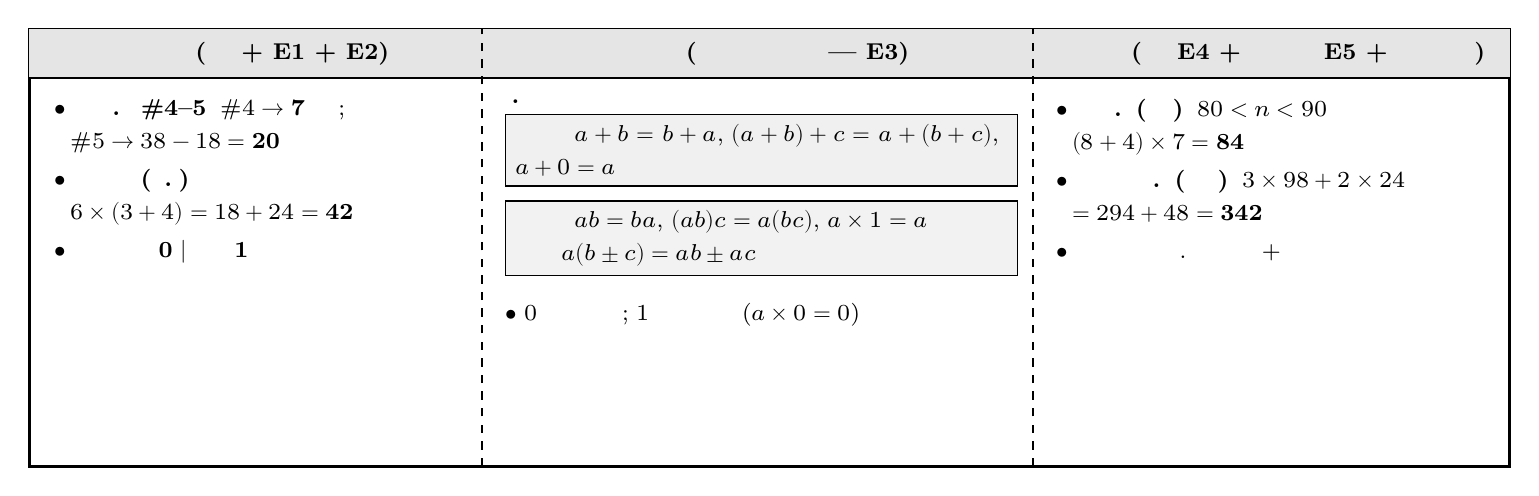
\begin{tikzpicture}[x=1cm, y=1cm, every node/.style={font=\fontsize{8.3pt}{11.8pt}\selectfont, text=black}]
  \draw[black, line width=1.1pt] (0,0) rectangle (18.8,5.55);
  \fill[gray!20] (0,4.93) rectangle (18.8,5.55);
  \draw[black, line width=0.7pt] (0,4.93) -- (18.8,4.93);
  \draw[black, dashed, line width=0.7pt] (5.75,0) -- (5.75,5.55);
  \draw[black, dashed, line width=0.7pt] (12.75,0) -- (12.75,5.55);

  \node at (2.875,5.24) {\textbf{ផ្នែកឆ្វេង (កំណែ + \en{E1} + \en{E2})}};
  \node at (9.25,5.24) {\textbf{ផ្នែកកណ្ដាល (ខ្លឹមសារគោលរក្សាទុក — \en{E3})}};
  \node at (15.775,5.24) {\textbf{ផ្នែកស្ដាំ (គំរូ \en{E4} + ប្រតិបត្តិ \en{E5} + កិច្ចការផ្ទះ)}};

  % Left
  \node[anchor=north west, text width=5.35cm] at (0.20,4.78) {%
    $\bullet$ \textbf{កំណែទំ.១៤ \#4–5៖} $\#4 \to \mathbf{7}$ ផ្លែ;\\
    \hspace*{0.2cm}$\#5 \to 38 - 18 = \mathbf{20}$ នាក់\\[2pt]
    $\bullet$ \textbf{ឧទាហរណ៍ ៣ (ទំ.៨)៖} ក្រឡាការ៉ូ\\
    \hspace*{0.2cm}$6 \times (3+4) = 18 + 24 = \mathbf{42}$\\[2pt]
    $\bullet$ ធាតុណឺតបូកគឺ $\mathbf{0}$ $\mid$ គុណគឺ $\mathbf{1}$
  };

  % Center
  \node[anchor=north west, text width=6.65cm] at (5.92,4.78) {%
    {\muol\fontsize{8.5pt}{12pt}\selectfont ៥\enbf{.} លក្ខណៈនៃប្រមាណវិធីបូកនិងគុណ}\\[3pt]
    \tikz\node[draw=black, fill=gray!12, inner sep=3.5pt, text width=6.25cm]{%
      វិធីបូក៖ $a+b=b+a$, $(a+b)+c=a+(b+c)$, $a+0=a$
    };\\[4pt]
    \tikz\node[draw=black, fill=gray!10, inner sep=3.5pt, text width=6.25cm]{%
      វិធីគុណ៖ $ab=ba$, $(ab)c=a(bc)$, $a\times 1=a$\\
      បំបែក៖ $a(b\pm c) = ab \pm ac$
    };\\[4pt]
    $\bullet$ $0$ ជាធាតុណឺតបូក; $1$ ជាធាតុណឺតគុណ ($a\times 0 = 0$)
  };

  % Right
  \node[anchor=north west, text width=5.65cm] at (12.92,4.78) {%
    $\bullet$ \textbf{គំរូទំ.៨ (ឃ្លី)៖} $80<n<90$\\
    \hspace*{0.2cm}$(8+4)\times 7 = \mathbf{84}$ គ្រាប់\\[2pt]
    $\bullet$ \textbf{ប្រតិបត្តិទំ.៩ (ក្រូច)៖} $3\times 98 + 2\times 24$\\
    \hspace*{0.2cm}$= 294 + 48 = \mathbf{342}$ ផ្លែ\\[2pt]
    $\bullet$ \textbf{កិច្ចការផ្ទះ៖} ទំ.១៤ លេខ ២ ក + ៣ ខ្ទង់
  };
\end{tikzpicture}
\end{center}

\vfill
\secstrip{២. ចម្លើយផ្ទៀងផ្ទាត់រហ័សសម្រាប់សន្លឹកកិច្ចការសិស្ស \enbf{(}ទំព័រ ១ និង ទំព័រ ២\enbf{)}}{\en{Answer Key}}

\begin{tcolorbox}[
  enhanced, sharp corners, colback=white, colframe=black,
  boxrule=0.8pt, boxsep=2.5pt, top=4.5pt, bottom=4.5pt, left=6pt, right=6pt
]
  \fontsize{9.0pt}{13.5pt}\selectfont
  $\bullet$ \textbf{ផ្នែក \en{E1}៖} \textbf{សិស្ស ខ} ត្រឹមត្រូវ ($42$ ការ៉ូ) ព្រោះកត្តា $6$ ត្រូវគុណនឹងតួក្នុងវង់ក្រចកទាំង $2$ តួ ($6\times 7 = 42$) ។\\[2pt]
  $\bullet$ \textbf{ផ្នែក \en{E2}៖} \textbf{សកម្មភាព ១៖} វិធីបូក $9, 10, 1$; វិធីគុណ $35, 60, 14$ ។ \textbf{សកម្មភាព ២៖} $6\times 7 = 42$; $18 + 24 = 42$; $(6\times 3)+(6\times 4)$ ។\\[2pt]
  $\bullet$ \textbf{ផ្នែក \en{E4}៖} $n=81 \to 63$; $n=84 \to 12\times 7 = \mathbf{84}$ គ្រាប់ ។ \en{EIA}៖ $12\times 7 = 70 + 14 = 84$ ។\\[2pt]
  $\bullet$ \textbf{ផ្នែក \en{E5}៖} \textbf{១) ប្រតិបត្តិទំ.៩៖} $(300-6)+(40+8) = 294 + 48 = \mathbf{342}$ ផ្លែ ។ \textbf{២) បិទ \en{E1}៖} សិស្ស ខ ($42$) ។ \textbf{៣) វិនិច្ឆ័យ \en{A--D}៖} \textbf{ជម្រើស \en{B}} ($80+40$) ។ \textbf{៤) សំបុត្រចេញ៖} $27\times(64+36) = 27\times 100 = \mathbf{2\,700}$ ។
\end{tcolorbox}

\vfill
\secstrip{៣. ចម្លើយលម្អិតនៃកិច្ចការផ្ទះ \enbf{(}សៀវភៅគោល ទំ.១៤ លេខ ២ ក និងលំហាត់គណនារហ័ស\enbf{)}}{សៀវភៅគោល ទំ.១៤}

\begin{tcolorbox}[
  enhanced, sharp corners, colback=white, colframe=black,
  boxrule=0.8pt, boxsep=2.5pt, top=4.5pt, bottom=4.5pt, left=6pt, right=6pt
]
  \fontsize{8.9pt}{13.3pt}\selectfont
  $\bullet$ \textbf{១) ទំ.១៤ លេខ ២ ក៖} $40 \times 5 + 50 \times 6 - 7 \times 60 = 200 + 300 - 420 = 500 - 420 = \mathbf{80}$ ។\\[2pt]
  $\bullet$ \textbf{២) គណនារហ័ស៖} ក. $25\times 19\times 4 = (25\times 4)\times 19 = 100\times 19 = \mathbf{1\,900}$; \quad ខ. $37\times(64+36) = 37\times 100 = \mathbf{3\,700}$; \quad គ. $6\times(100-1) = 600-6 = \mathbf{594}$ ។
\end{tcolorbox}

\vfill
\secstrip{៤. ចំណុចប្រុងប្រយ័ត្នគរុកោសល្យសម្រាប់គ្រូ \enbf{(}ការយល់ច្រឡំសំខាន់ៗរបស់សិស្ស\enbf{)}}{\en{Pedagogical Watchlist}}

\begin{tcolorbox}[
  enhanced, sharp corners, colback=panelgray, colframe=black,
  boxrule=0.85pt, boxsep=2.5pt, top=4.5pt, bottom=4.5pt, left=6pt, right=6pt
]
  \fontsize{8.8pt}{13.1pt}\selectfont
  $\bullet$ \textbf{អន្ទាក់គុណតែតួទី១ ក្នុងវង់ក្រចក (\en{Ding \& Li, 2014})៖} បើសិស្សសរសេរ $6\times(3+4) = 6\times 3 + 4$ ចូរឱ្យសិស្សចង្អុលរាប់ជួរដេកលើរូបក្រឡាការ៉ូទំ.៨ ដើម្បីឃើញថាក្រឡាផ្នែកស្ដាំមាន $6\times 4 = 24$ ការ៉ូ មិនមែន $4$ ការ៉ូទេ!\\[2pt]
  $\bullet$ \textbf{អន្ទាក់ធាតុណឺតនៃវិធីគុណ (\en{Larsen, 2010})៖} សង្កត់ធ្ងន់ថា $0$ ជាធាតុណឺតនៃវិធីបូក ($a+0=a$) រីឯ $1$ ជាធាតុណឺតនៃវិធីគុណ ($a\times 1=a$) ចំណែក $a\times 0 = 0$ ។
\end{tcolorbox}

\end{document}
